\chapter{Compositie en aggregatie.} 
\label{ch:hfstCompAgg}
Bij deze opdracht worden aggregatie en compositie in C++ geïmplementeerd. Met behulp van de DDD debugger worden objecten en hun onderlinge verbindingen zichtbaar gemaakt. Hiervan zullen verschillende screenshots gemaakt moeten worden die opgenomen  moeten worden in je portfolio. De portfolio moet aan het einde van de week geüpload worden op Brightspace. Tijdens het aftekenen moeten de screenshots zichtbaar zijn. Op de screenshots zal je \textbf{eigen} \textcolor{BrickRed}{\textbf{naam}} en \textcolor{BrickRed}{\textbf{studienummer}} moeten staan.

De opdracht bestaat uit een speciaal type LED, de Logled. De Logled heeft als extra een Stopwatch en een Tijdsduur. De klasse wordt weergegeven in Figuur \ref{fig:logled}.
    \begin{figure}[h!]
	\captionsetup{justification=centering}
	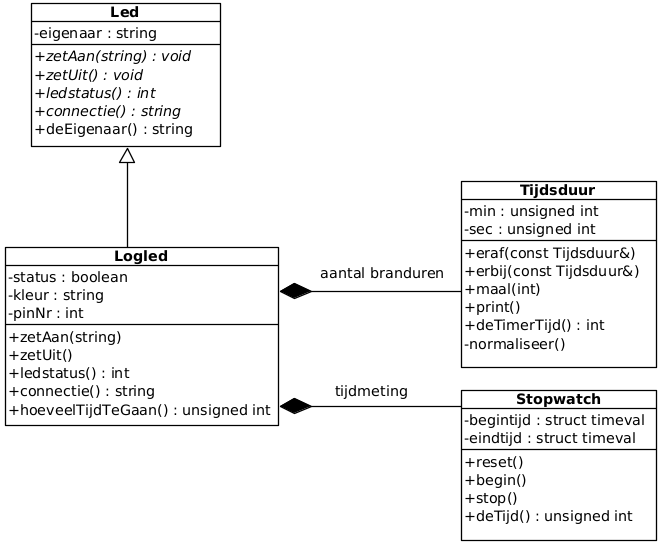
\includegraphics[width=0.9 \linewidth]{figuren/logled}      %ledPlatform}
\centering
\caption{De logled met timer en stopwatch.}
\label{fig:logled}
\end{figure} 
De Logled is speciaal ontwikkeld om ervoor te zorgen dat een maximale levensduur voor de LED kan worden ingesteld. Daarna moet een nieuwe Logled gekocht worden. 
\begin{itemize}
	\item Met de tijdsduur wordt bijgehouden hoeveel minuten de Logled nog aan mag. 
	\item Met de stopwatch wordt elke keer gecheckt hoe lang de Logled voor dat moment aan is.
	\item De Led uit de vorige opgave kan hergebruikt worden. De stopwatch krijg je cadeau en is te downloaden van Github. \\De klasse Logled en Tijdsduur moet je zelf maken.
\end{itemize}

\section{De klasse Tijdsduur.}

We willen een ADT (Abstract Data Type) , ook wel zelfgedefinieerd datatype genoemd, maken waarin een tijdsduur in minuten en seconden kan worden opgeslagen. De totale tijd in seconden kan ook worden opgevraagd. 
\begin{figure}[h!]
	\captionsetup{justification=centering}
	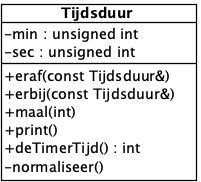
\includegraphics[width=0.28 \linewidth]{figuren/tijdsduur}
	\centering
	\caption{weergave van de klasse Tijdsduur. }
	\label{fig:tijdsduurKlas}
\end{figure}
We noemen dit zelf gedefinieerde datatype \texttt{Tijdsduur}. Figuur \ref{fig:tijdsduurKlas} geeft de klasse weer van Tijdsduur.
Het ADT \texttt{Tijdsduur} kan in C++ als volgt gedeclareerd worden in de header file (tijdsduur.h):

\begin{lstlisting}[caption= de headerfile van de klasse \texttt{Tijdsduur},label={lst:tijdsdHeader},numbers=none]		
	#ifndef TIJDSDUUR_H
	#define TIJDSDUUR_H
	
	// De declaratie van de ADT Tijdsduur:
	class Tijdsduur {
		public:
		//...
		void eraf(Tijdsduur t);
		//...
		
		private:
		int sec;
		//...
	};
	#endif // TIJDSDUUR_H
\end{lstlisting}

De implementatie (\texttt{tijdsduur.cpp}) ziet er tot nu toe als volgt uit:
\begin{lstlisting}[caption= de implementatiefile van de klasse \texttt{Tijdsduur},label={lst:tijdsdImpl},numbers=none]
	#include <iostream>
	#include "tijdsduur.h"
	#include <iomanip>
	using namespace std;
	
	// De definities van de memberfunctie van de ADT Tijdsduur, oftewel: de implementatie van de ADT Tijdsduur:
	void Tijdsduur::eraf(Tijdsduur t) {
		sec-=t.sec;
		//...
	}
\end{lstlisting}

Het hoofdprogramma (\texttt{opg13.cpp}) ziet er als volgt uit:

\begin{lstlisting}[caption= de implementatiefile van het hoofdprogramma ,label={lst:tijdsdMainprog},numbers=none]
	#include <iostream> // nodig voor cout (schrijven naar scherm)
	#include <iomanip> // nodig voor setw (veldbreedte definieren )
	#include "tijdsduur.h"
	using namespace std;
	
	int main() {
		Tijdsduur t1(3,50); // t1 is 3 minuten en 50 seconden
		cout<<"t1 = "; t1.print(); cout<<endl;
		const Tijdsduur kw(15); // kw is 15 seconden
		cout<<"kw = "; kw.print(); cout<<endl;
		t1.erbij(kw); // Tel kw bij t1 op
		cout<<"t1 = "; t1.print(); cout<<endl;
		Tijdsduur t2(t1); // t2 is een kopie van t1
		t2.eraf(kw); // Trek kw van t2 af
		cout<<"t2 = "; t2.print(); cout<<endl;
		t2.maal(7); // Vermenigvuldig t2 met 7
		cout<<"t2 = "; t2.print(); cout<<endl;
		Tijdsduur t3(3,-122); // t3 is 3 minuten minus 122 seconden
		cout<<"t3 = "; t3.print(); cout<<endl;
		t3.eraf(t2); 
		cout<<"t3 = "; t3.print(); cout<<endl;
		Tijdsduur t4(3,122); // t4 is 3 minuten plus 122 seconden
		cout<<"t4 = "; t4.print(); cout<<endl;
		cout<<"het totaal aantal seconde van t4 = "<<t4.deTimerTijd()<<endl;
		return 0;
	}	
\end{lstlisting}
De uitvoer moet dan zijn:

\begin{tabular}{ l l l }
	t1= & 3 minuten en & 50 seconden \\ 
	kw	=& &15	seconden \\  
	t1	=&	4	minuten en&	5	seconden\\
	t2	=&	3	minuten en	&50	seconden\\
	t2	=&	26	minuten en	&50	seconden\\
	t3	=&			&58	seconden\\
	t3	=&			&0	seconden\\
	t4	=&	5	minuten en	&2	seconden
	
\end{tabular}

\paragraph{Opdracht}
\begin{enumerate}[label=\alph*]
	\item De code van de implementatie van de klasse tijdsduur, zoals hierboven vermeld is, is verre van compleet.
	Download  opg13.zip van Brightspace of clone deze:\\ 
	{\small \texttt{git clone } \verb|--| \texttt{branch logled https://github.com/JohnVi-hhs/oop.git}}
	
	Vul de declaratie en de implementatie van de ADT genaamd  Tijdsduur verder in. Zorg ervoor dat het hoofdprogramma (\texttt{testTijdsduur.cpp}) zonder warnings te compileren is en de gewenste uitvoer produceert. Zoek (indien nodig) inspiratie bij de in de les behandelde \texttt{\textbf{class} Breuk}. Tip: Zorg ervoor dat de opgeslagen seconden altijd \textgreater =0 en \textless 60 zijn.
	\item Voer zelf nog een aantal testen met Tijdsduur uit. B.v het gebruik van de methode\texttt{ int deTimerTijd()}.
	\item Laat de opdracht aftekenen.
\end{enumerate}


\section{De klasse Logled}

Zoals uit Figuur \ref{fig:logled} blijkt heeft de klasse \textbf{Logled} twee compositie klassen, namelijk de klassen \textbf{Tijdsduur} en \textbf{Stopwatch}.
Hierdoor kan het maximum aan minuten en seconden dat een Logled in totaal aan kan gaan, worden opgegeven. Stel een Logled wordt gecreëerd met de volgende regel:
\begin{lstlisting}
	Logled logger(135,"rood","Pietje Puk",0,4);
\end{lstlisting}
Dit houdt in dat een Logled wordt aangemaakt met als naam \texttt{logger}. De led wordt aangesloten op pin 135 en heeft de kleur rood. De eigenaar is "Pietje Puk". De maximale tijd dat een led in totaal aan kan gaan is 0 minuten en 4 seconden.
De werking van de methoden \texttt{zetAan} en \texttt{zetUit} van Logled zijn als volgt:

\begin{itemize}
	\item De methode \texttt{void zetAan("groen");}  
	  \begin{enumerate}
	  	\item Er wordt gecontroleerd of de meegegeven kleur overeenkomt met de kleur van de led.
	  	\begin{itemize}
	  		\item Nee: return.
	  		
	  	\end{itemize}
	  	\item De tijd dat de led nog aan mag, wordt opgehaald.
	  	\item Opgehaalde tijd \textgreater  0 ?
	  		  	\begin{enumerate}
	  		\item Reset de stopwatch.
	  		\item Begin met tijdmeting.
	  		\item Zet de led aan.	  		
	  	\end{enumerate}
	  \end{enumerate}
  In het sequentiediagram van Figuur \ref{fig:ll_zetAan} wordt een scenario weergegeven wanneer de Logled aangezet wordt en 
      \begin{figure}[h!]
  	\captionsetup{justification=centering}
  	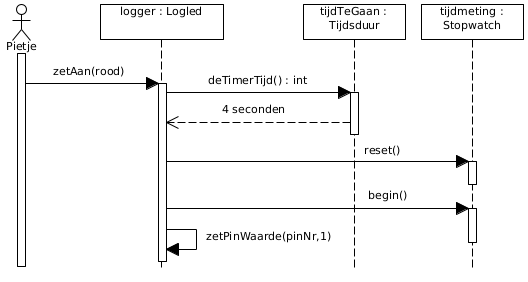
\includegraphics[width=0.8 \linewidth]{figuren/seqZetAan}      %ledPlatform}
  \centering
  \caption{De werking van de methode zetAan.}
  \label{fig:ll_zetAan}
\end{figure} 
 deze nog 4 seconden te gaan heeft. 

 \item De methode \textit{void zetUit()} doet het volgende: 
 \begin{itemize}
 	\item Stop de stopwatch.
 	\item Haal de stopwachttijd op.
 	\item Breng deze tijd in mindering bij tijdTeGaan.
 	\item Zet de led uit.
 \end{itemize} 
 In het sequentiediagram van Figuur \ref{fig:ll_zetUit} wordt een scenario weergegeven wanneer de Logled wordt uitgezet
  \begin{figure}[h!]
	\captionsetup{justification=centering}
	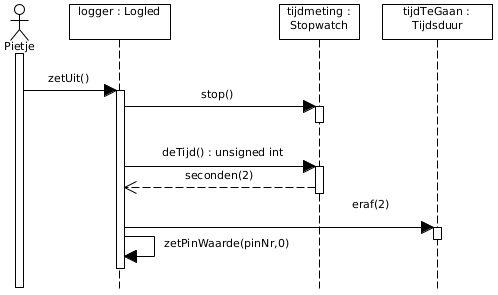
\includegraphics[width=0.8 \linewidth]{figuren/seqZetUit}      %ledPlatform}
\centering
\caption{De werking van de methode zetUit.}
\label{fig:ll_zetUit}
\end{figure} 
nadat deze 2 seconden heeft aangestaan.
\end{itemize}
\newpage
\paragraph{Opdracht}

\begin{enumerate}[label=\alph*]
	\item Implementeer de klasse Logled, zodat de code van listing \ref{lst:loglImpl} zonder compiler errors en warnings werkt.
	\begin{lstlisting}[caption=Een test van de klasse \texttt{LogLed}. ,frame=trbl,firstnumber=1,numbers=left,label={lst:loglImpl}]{Name}
#include <iostream> // nodig voor cout (schrijven naar scherm)
#include <unistd.h>
#include "Logled.h"

using namespace std;

#define RODELEDPIN 135
#define GROENELEDPIN 132

#define TWEE_SEC 2000000
#define DRIE_SEC 3000000

int main() {
	//Een object van de klasse Logled met een maximale 'aan' tijd van 2 seconde 
	Logled logger(RODELEDPIN,"rood","Pietje Puk",0,2);
	logger.zetAan("rood");
	usleep(DRIE_SEC); //wacht 3 seconden
	ll1.zetUit();
	logger.zetAan("rood");//led gaat niet meer aan.
	return 0;
}	
\end{lstlisting}
\item  Pas de \texttt{main()} aan zodat deze eruit ziet als listing \ref{lst:logled2}
\begin{lstlisting}[caption=Twee objecten van de klasse \texttt{LogLed}. ,frame=trbl,firstnumber=1,numbers=left,label={lst:logled2}]{Name}
int main() {
	
	Logled logger(RODELEDPIN,"rood","Pietje Puk",0,4);
	Logled sportled(GROENELEDPIN,"groen","Bb",0,2);
	
	logger.zetAan("rood");
	sportled.zetAan("groen");
	usleep(DRIE_SEC); //wacht 3 seconden
	logger.zetUit();
	sportled.zetUit();
	usleep(TWEE_SEC);//wacht 2 seconden
	logger.zetAan("rood");
	sportled.zetAan("groen");
	usleep(TWEE_SEC);//wacht 2 seconden
	logger.zetUit();
	sportled.zetUit();
	
	return 0;
}	
\end{lstlisting}
Compileer het programma en laat het runnen. Plaats de code (\texttt{.h} en \texttt{.cpp}) file van de klasse \textbf{Logled} in je portfolio.
\newpage
\item Open de VNC viewer, run de DDD debugger (\texttt{ddd ./testlogled}), zet een breakpoint bij het statement  \texttt{usleep(TWEE\_SEC);} (regel 11 van listing \ref{lst:logled2})
\begin{figure}[h!]
\captionsetup{justification=centering}
	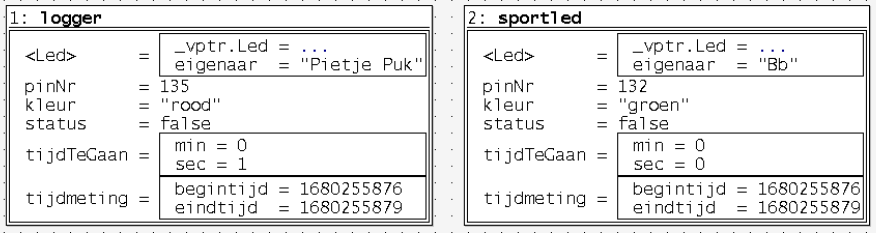
\includegraphics[width=0.85 \linewidth]{figuren/dddTweeLogleds}      
\centering
\caption{Twee objecten van de klasse Logled}
\label{fig:dddTweeLogl}
\end{figure}
en display beide objecten (\texttt{logger} en \texttt{sportled}) van de klasse \textbf{Logled}. Als het goed is krijg je iets te zien zoals Figuur \ref{fig:dddTweeLogl}, uiteraard met je \textcolor{red}{eigen} naam.\\
Maak van de afbeelding een screenshot en plaats deze in je portfolio.
\item Voer het programma nog een keer uit en maak gedurende de uitvoer twee \textcolor{BlueViolet}{\textbf{screenshots}} die lijken op Figuur \ref{fig:logledOjecten}. Indien Args niet zichtbaar is, kan deze zichtbaar gemaakt worden via Data $\rightarrow$	 Display Arguments (ALT + U).
Led op: De begintijd van \ref{fig:logObjectA} en \ref{fig:logObjectB} zijn hetzelfde, de stopwatch is immers een compositie van Logled.
\begin{figure}[h!]
	\centering
	\begin{center} 	
		\begin{subfigure}[b]{0.49\textwidth}
			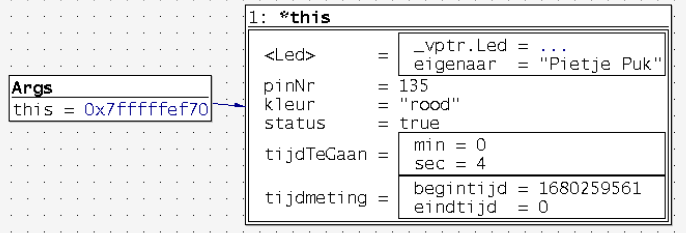
\includegraphics[width=0.95\textwidth]{figuren/ddd_logled_p2a}
			\caption{Logled met composities Tijdsduur en Stopwatch.}
			\label{fig:logObjectA}
		\end{subfigure}
		\begin{subfigure}[b]{0.49\textwidth}
			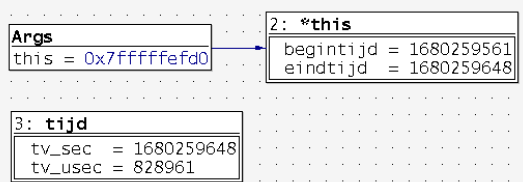
\includegraphics[width=0.95\textwidth]{figuren/ddd_logled_p2b}
			\caption{Van het object stopwatch, de attributen en lokale variabele tijd.}
			\label{fig:logObjectB}
		\end{subfigure}
		\caption{Inhoud van het object Logled bij het aanroepen van de zetUit() en vervolgens stap voor stap naar methode stop() van stopwatch.}
		\label{fig:logledOjecten}   
	\end{center}
\end{figure}
Bij Figuur \ref{fig:logObjectB} zie je de waarde van de attributen van het object van de klasse \textit{Stopwatch} waarbij \textit{\textbf{tijd}} een lokale variabele is binnen de methoden \textit{void begin()} en \textit{void stop()} van de klasse Stopwatch.
\end{enumerate}



